\documentclass[14pt,xcolor=dvipsnames]{beamer}
\usepackage{tikz}
\usepackage{pgfplots}
\usetikzlibrary{shapes,arrows}
\hypersetup{
    colorlinks=true,
    linkcolor=blue,
    filecolor=magenta,      
    urlcolor=blue,
    pdftitle={Overleaf Example},
    pdfpagemode=FullScreen,
    }
\pgfplotsset{compat=1.17}
\usefonttheme{professionalfonts}
\usetikzlibrary{shapes,arrows}
\newcommand{\mx}[1]{\mathbf{\bm{#1}}} % Matrix command
\newcommand{\vc}[1]{\mathbf{\bm{#1}}} % Vector command
\usepackage{amsmath,enumerate,xspace,bbold,amsthm,arydshln,bm}
\usepackage{multirow,array,theorem,amsmath,latexsym,xspace, bibentry,tikz}
\usepackage{array,theorem,amsmath,latexsym,hhline,pifont,xspace, bibentry,epstopdf, comment,dsfont}
%\usepackage{algorithm,algorithmic,comment}
\usepackage{algorithm,algpseudocode}
\usepackage[round,authoryear]{natbib}
\usepackage{grffile}
\usepackage{booktabs}
\usepackage{graphicx}
\usetikzlibrary{tikzmark,arrows}
\usetikzlibrary{positioning,arrows.meta}
\usetheme{AnnArbor}
\setbeamerfont*{itemize/enumerate subbody}{parent=itemize/enumerate body}
\setbeamerfont*{itemize/enumerate subsubbody}{parent=itemize/enumerate body}
\setbeamercolor{alerted text}{fg=red!80!yellow}
\newcommand{\libsvm}{$\mbox{\href{http://www.csie.ntu.edu.tw/~cjlin/libsvm}{\sf LIBSVM}}$\xspace}
\newcommand{\liblinear}{$\mbox{\href{http://www.csie.ntu.edu.tw/~cjlin/liblinear}{\sf LIBLINEAR}}$\xspace}
\usetikzlibrary{matrix}
\usetikzlibrary{fit}
\usetikzlibrary{calc}
\usetikzlibrary{decorations.pathreplacing}
\def\R{{ \mathbf{R}}}
\def\Z{{ \mathbf{Z}}}
\def\ba{{\boldsymbol a}}
\def\bc{{\boldsymbol c}}
\def\bg{{\boldsymbol g}}
\def\bt{{\boldsymbol t}}
\def\bx{{\boldsymbol x}}
\def\by{{\boldsymbol y}}
\def\bi{{\boldsymbol I}}
\def\br{{\boldsymbol r}}
\def\bz{{\boldsymbol z}}
\def\bv{{\boldsymbol v}}
\def\bb{{\boldsymbol b}}
\def\bp{{\boldsymbol p}}
\def\bq{{\boldsymbol q}}
\def\bw{{\boldsymbol w}}
\def\bu{{\boldsymbol u}}
\def\bv{{\boldsymbol v}}
\def\bs{{\boldsymbol s}}
\def\be{{\boldsymbol e}}
\def\bd{{\boldsymbol d}}
\def\b1{{\boldsymbol 1}}
\def\bk{{\boldsymbol k}}
\def\bzero{{\boldsymbol 0}}
\def\btheta{\boldsymbol \theta}
\def\bxi{\boldsymbol \xi}
\def\AL{{\boldsymbol{\alpha}}}
\def\ALL{{\boldsymbol{\alpha'}}}
\def\BL{\boldsymbol \beta}
\def\boldgamma{\boldsymbol \gamma}
\def\bla{\boldsymbol \lambda}
\def\bnu{\boldsymbol \nu}
\def\bmu{\boldsymbol \mu}
\def\boldeta{\boldsymbol \eta}
\def\tron{{\sf TRON}\xspace}
\def\vec{{\text{vec}}}
\def\mat{{\text{mat}}}
\def\mfirst{m}
\def\msec{{m+1}}
\def\mQ{\mathbf{Q}}
\def\mK{\mathbf{K}}
\def\mV{\mathbf{V}}
\def\mO{\mathbf{O}}
\def\mS{\mathbf{S}}
\def\mP{\mathbf{P}}
% Force numbering to start from 0
\setcounter{algorithm}{-1}

\setbeamertemplate{caption}[numbered]

\newcommand{\rom}[1]{\uppercase\expandafter{\romannumeral #1\relax}}
\AtBeginSection[]
{
	\begin{frame}<beamer>
		\frametitle{Outline}
		\tableofcontents[current,currentsection]
	\end{frame}
}

\tikzset{
    neuron/.style={circle, line width=1.2pt, draw, minimum size=8mm},
    crossed/.style={circle, line width=1.2pt, draw, minimum size=8mm, dashed},
    connect/.style={-latex, line width=1.2pt},
}

\begin{document}
	\tikzset{
		arr/.style={draw opacity=1,
			decoration={markings,mark=at position 1
				with {\arrow[scale=2]{>}}},
			postaction={decorate}, shorten >=0.4pt,
		}
	}
	
	% \title[]{Some Notes on Automatic Differentiation}
	% \author[Chih-Jen Lin]{{\large Chih-Jen Lin}\\
	% 	% Department of Computer Science\\
	% 	National Taiwan University \\
	% 	\bigskip
	% 	Last updated: \today
	% 	%\centering\epsfig{figure = ../../ntulogo.eps, width = 2.5cm} 
	% 	%\includegraphics[width=1.85cm]{./ntulogo.png}
	% 	% \\
	% 	% {\small 
	% 	% Joint work with Chien-Chih Wang, Kent Loong Tan, Chun-Ting
	% 	% Chen (National Taiwan University), and Sathiya Keerthi, Dhruv
	% 	% Mahajan, Sundararajan Sellamanickam (Microsoft)
	% 	% }
	% }
	
	% \institute[National Taiwan Univ.]{}
	% \date[]{}
	% % \begin{frame}
	% %    \titlepage
	% % \end{frame}
	% %\logo{\includegraphics[width=0.5cm]{../../../latex/ntulogo.png}}

\title[]{An Introduction to FlashAttention}
\author[Chih-Jen Lin]{{\large Chih-Jen Lin}\\
% Department of Computer Science\\
National Taiwan University, MBZUAI \\
\bigskip
Last updated: \today
}

\institute[National Taiwan Univ.]{}
\date[]{}
\begin{frame}
   \titlepage
\end{frame}

%\begin{frame}
%  \frametitle{Outline}
%  \tableofcontents[hideallsubsections]
%\end{frame}

\begin{frame}[allowframebreaks]
	\frametitle{Inefficiency of Attention Operation}
	\begin{itemize}
		\item Similar to the memory-access issue discussed
          above for matrix-matrix products, a
          possible bottleneck of attention is
          on moving data (i.e., matrices) between
          lower-level and upper-level memory on GPUs.
        \item To analyze this issue, we must check the number
          of memory accesses.
	\end{itemize}
\end{frame}

\begin{frame}[allowframebreaks]
  \frametitle{Attention Operations}
  \begin{itemize}
  \item For the discussion, first we recall details
    of attention. For simplicity, we consider
    the single-head attention.
\item If the input matrix is
  \begin{equation*}
    \tilde{Z} \in \R^{T \times d},
  \end{equation*}
  the attention operation is
    \begin{equation}
      \label{eq:attention1}
\text{SoftMax} (\frac{\tilde{Z} W_Q W_K^\top (\tilde{Z})^\top}{\sqrt{d}}) \tilde{Z} W_V.
    \end{equation}
  \item We consider three
 trainable weight matrices
    \begin{equation*}
      W_Q \in \R^{d \times d}, W_K \in \R^{d \times d}, W_V \in \R^{d \times d}
    \end{equation*}
    to convert the input matrix $\tilde{Z}$ to
    \begin{equation*}
\tilde{Z} W_Q \in \R^{T\times d}, \quad \tilde{Z} W_K \in \R^{T\times d}, \quad \tilde{Z} W_V \in \R^{T\times d}.
\end{equation*}
  \item In \eqref{eq:attention1}, the \text{SoftMax} function
    is applied on each row $\bz$ of an input matrix in 
the following way.
    \begin{equation}
      \label{eq:softmax}
      \text{SoftMax}(\textbf{z}) = \begin{bmatrix} \frac{\exp(z_1)}{\sum_j\exp(z_j)}\\\vdots\\\frac{\exp(z_T)}{\sum_j\exp(z_j)}\end{bmatrix}.
    \end{equation}
  \item FlashAttention \citep{TD22a} defines that
  \begin{equation*}
  	\mQ := \tilde{Z} W_Q, \quad \mK := \tilde{Z} W_K, \quad \mV := \tilde{Z} W_V,
  \end{equation*}
  and assumes that $\mQ, \mK, \mV$ had been already precomputed.
  \item Omitting $1/\sqrt{d}$ for simplification, FlashAttention turns \eqref{eq:attention1} into
  \begin{equation}
  \label{eq:attention2}
  	\mO := \text{SoftMax} (\mQ \mK^\top) \mV,
  \end{equation}
  where $\mO \in \R^{T\times d}$ is the output matrix of the attention.
  \end{itemize}
\end{frame}


\begin{frame}[allowframebreaks]
  \frametitle{Memory Accesses in Attention}
  \begin{itemize}
  \item We still assume that our machine has
only two layers of memory:
  \begin{itemize}
  \item main memory, and
  \item secondary memory.
  \end{itemize}
\item If an operand is not 
available in main memory, we must transport it from secondary 
memory.
\item Now consider \eqref{eq:attention2} and check intermediate
  values during computation.
\item We need
  \begin{gather}
\mQ \mK^\top \in R^{T \times T}, \label{eq:attention_op1}\\
\text{SoftMax} (\mQ \mK^\top) \in R^{T \times T},
\label{eq:attention_op2}\\
\text{SoftMax} (\mQ \mK^\top) \mV \in R^{T \times d}.
\label{eq:attention_op3}
  \end{gather}
\item As in general
  \begin{equation*}
    T \gg d,
  \end{equation*}
even though the output
  \begin{equation*}
    \text{SoftMax} (\mQ \mK^\top) \mV \in R^{T \times d}
  \end{equation*}
is smaller,  storing $T\times T$ intermediate matrices is the main
  difficulty.
  \end{itemize}
\end{frame}

\begin{frame}[allowframebreaks]
\frametitle{Insufficient Memory to Store $T \times T$
  Intermediate Matrices}
  \begin{itemize}
\item Our first analysis is to assume that
  \begin{equation*}
    T \times T
  \end{equation*}
  matrices cannot be stored in the main memory, and check the
  need to move these matrices
\item If we consider
  \eqref{eq:attention_op1}-\eqref{eq:attention_op3} as
  independent operations, immediately we see the following
  major memory accesses:
  \begin{itemize}
  \item write
    \begin{equation}\label{eq:attention_mat1}
\mQ \mK^\top \in R^{T \times T}
\end{equation}
to secondary memory,
\item load the matrix \eqref{eq:attention_mat1} from secondary memory to calculate
  \begin{equation}
    \label{eq:attention_mat2}
\text{SoftMax} (\mQ \mK^\top) 
\end{equation}
and write results back to secondary memory, and
\item load the matrix in \eqref{eq:attention_mat2}
  for calculating 
  \begin{equation*}
\text{SoftMax} (\mQ \mK^\top) \mV \in R^{T \times d}.
\end{equation*}
\end{itemize}
\item We assume that even though storing an $T\times T$
  matrix in main memory is not possible, the computer has
  a way to sequentially work on part of the
  input data in main memory and gradually generate/save part of the whole output to secondary memory
\item [] It is just like that we do matrix-matrix products
  all the time, but never worry that our highest-level
  memory (i.e., registers) is insufficient to store
  operands.
\item Now we conclude that a naive implementation of attention
  leads to
  \begin{equation}
    \label{eq:4Tsq}
    4 \times T^2
  \end{equation}
  accesses between main and secondary memory.
  \end{itemize}
\end{frame}

\begin{frame}[allowframebreaks]
	\frametitle{Memory Versus Computation}
        \begin{itemize}
        \item We see attention involves the following
          operations and list their respective cost.
  \begin{gather*}
\mQ \mK^\top: 2 T^2 d, \\
\text{SoftMax} (\mQ \mK^\top): 3T^2,
\\
\text{SoftMax} (\mQ \mK^\top) \mV: 2T^2d.
  \end{gather*}
\item Clearly, if
  \begin{gather*}
    4T^2 d \times \text{ cost per operation}\\
    <
    \\
    4T^2 \times \text{ cost per memory access},
  \end{gather*}
  then attention is \alert{memory bounded}.
\item Example:
  \begin{itemize}
    \item Consider $T=1024$ and $d=64$, running on an A100 80GB SXM GPU. 
    \item This GPU sustains up to 312 tera floating point operations per second (TFLOPS) for half-precision floating-point format (FP16) operations.
    \item The GPU is equipped with 80 GB of high-bandwidth memory (HBM), corresponding to the secondary memory in our setting and offering a memory bandwidth of 2.04 tera bytes per second (TB/s).
    \item Then, the total compute cost is
    \begin{equation*}
      \frac{4 \times 1024^2 \times 64 \ \text{FLOPs}}{312 \ \text{TFLOPS}} 
      \;\approx\; 0.86~\mu\text{s}.
    \end{equation*}
    \item The total memory access cost is
    \begin{equation*}
      \frac{4 \times 1024^2 \times 2 \ \text{bytes}}{2.04 \ \text{TB/s}} 
      \;\approx\; 3.74~\mu\text{s}.
    \end{equation*}
    Note that we assume each value is stored in FP16 (two bytes).
    % \item Clearly, $3.74~\mu\text{s} \gg 0.86~\mu\text{s}$, 
    % indicating that the runtime is dominated by memory accessing.
    % \item Thus, with FP16 operations on the A100 80GB SXM and $T=1024$, $d=64$, 
    % the attention layer is severely \textbf{memory-bounded}.
  \end{itemize}
\item To accelerate attention, we must reduce the number of memory accesses.
\end{itemize}
\end{frame}


\begin{frame}[allowframebreaks]
	\frametitle{Situation When Storing $T \times d$ Matrices Are Possible}
        \begin{itemize}
        \item Now we assume that the main memory is sufficient to store
          \begin{equation*}
            T\times d \text{ matrices such as }
            Q, K, \text{ and } V. 
          \end{equation*}
        \item Let us develop strategies to reduce the
          number of memory accesses in \eqref{eq:4Tsq}.
        \item In particular, we would like to avoid loading
          and storing intermediate results.
        \item That is, we should generate the attention
          results ``part by part.'' All we need is to
          sequentially store the finished part back
          to the secondary memory.
        \item We can conduct the following procedure:
\begin{itemize}
\item Load $Q, K, \text{ and } V$ to main memory.
\item For $i = 1, \ldots, T$, calculate
  \begin{gather}
\mQ_{i,:} \mK^\top \in R^{1\times T}, \label{eq:Nd1}\\
\text{SoftMax} (\mQ_{i,:} \mK^\top) \in R^{1\times T},\label{eq:Nd2}
\\
\text{SoftMax} (\mQ_{i,:} \mK^\top) \mV \in R^{1\times d}\label{eq:Nd3}
\end{gather}
and store the $i$th row of the output matrix to the secondary memory.
\end{itemize}
\item By this way, the number of memory accesses is reduced
  to
  \begin{equation*}
    O(Td).
  \end{equation*}
  because we never load/store any $T\times T$ matrices.
        \end{itemize}
\end{frame}


\begin{frame}[allowframebreaks]
	\frametitle{Situation When Storing $T \times d$ Matrices Are Not Possible}
        \begin{itemize}
\item Unfortunately, our assumption of that $T \times d$
  matrices can be stored in main memory is often untrue.
\item We discuss the situation of
  \begin{equation*}
    d \leq M \leq Td,
  \end{equation*}
    where $M$
  is the size of the main memory.

\item Then in \eqref{eq:Nd1}-\eqref{eq:Nd3}, we must load the
  whole $K$ and $V$ once
  even for calculating just one output row.
\item A possible strategy is to calculate $|I|$ rows together:
  \begin{equation}\label{eq:QK}
    \text{SoftMax} (\mQ_{I,:} \mK^\top) \mV,
  \end{equation}
  where $I$ is the block of rows that we intend to calculate.
\item In calculating \eqref{eq:QK}, we must access
  \begin{center}
    $|I|$ rows of $Q$, and the whole $K$ and $V$ (by row blocks). 
  \end{center}
  
\item We also need to store the intermediate block of
  \begin{equation}
    \label{eq:intermediate}
    \mQ_{I,:} \mK^\top,
  \end{equation}
  which requires
  \begin{equation*}
    |I| \times T
  \end{equation*}
  space.
\item The largest possible $|I|$ is
  \begin{equation*}
    \frac{M}{T},
  \end{equation*}
  where $M$
  is the size of the main memory.
\item Thus the total number of memory accesses is
  \begin{equation}
    O(\frac{T}{M/T}) \times O(Td)
    = O(\frac{T^3 d}{M}).\label{eq:Ncubic}
  \end{equation}
\item In the above discussion, we see that the main bottleneck is to
  store the intermediate matrix in \eqref{eq:intermediate}.
\item Because the number of rows in \eqref{eq:intermediate}
  is a large number $T$,
  $|I|$ must be small. Thus we get a large first term in \eqref{eq:Ncubic}.
        \end{itemize}
\end{frame}


\begin{frame}[allowframebreaks]
	\frametitle{FlashAttention}
        \begin{itemize}
\item To reduce the number of memory accesses, let us see if we may avoid storing the intermediate matrix in \eqref{eq:intermediate}.
\item Assume that we split $Q$ to the following row-block form:
  \begin{equation*}
    \begin{bmatrix}
      Q_{I_1,:}\\
      \vdots\\
      Q_{I_{T_r},:}
    \end{bmatrix}
  \end{equation*}
with
  \begin{equation*}
    |I_1| = \cdots = |I_{T_r}|.
  \end{equation*}
\item For $K, V$, we respectively split them to
    \begin{equation*}
    \begin{bmatrix}
      K_{J_1,:}\\
      \vdots\\
      K_{J_{T_c},:}
    \end{bmatrix},
        \begin{bmatrix}
      V_{J_1,:}\\
      \vdots\\
      V_{J_{T_c},:}
    \end{bmatrix}.
  \end{equation*}
\item We explain later why the split of $Q$ should be
  different from that of $K, V$.
\item In our discussion, we let $I, J$ be any one of
  $  |I_1|, \ldots, |I_{T_r}|$ and
    $  |J_1|, \ldots, |J_{T_c}|$, respectively.
  \item We have
    \begin{equation*}
      \begin{split}
&        \text{SoftMax} (\mQ_{I,:}
        \begin{bmatrix}
          \mK_{J_1,:}^\top & \cdots & \mK_{J_{T_c},:}^\top
        \end{bmatrix}
        )
        \begin{bmatrix}
          \mV_{J_1,:} \\ \vdots \\ \mV_{J_{T_c},:}
        \end{bmatrix}
  \\
        = &
        \text{SoftMax} (
        \begin{bmatrix}
          \mQ_{I,:}\mK_{J_1,:}^\top & \cdots & \mQ_{I,:}\mK_{J_{T_c},:}^\top
        \end{bmatrix}
        )
        \begin{bmatrix}
          \mV_{J_1,:} \\ \vdots \\ \mV_{J_{T_c},:}
        \end{bmatrix}
       \end{split}
    \end{equation*}
  \item If there is no SoftMax, we can see the result is
 \begin{equation*}
    (\mQ_{I,:}   \mK_{J_1,:}^\top)  \mV_{J_1,:} +
 \cdots + 
  (\mQ_{I,:}\mK_{J_{T_c},:}^\top) \mV_{J_{T_c},:}.
 \end{equation*}
\item We have
  \begin{gather*}
    (\mQ_{I,:}   \mK_{J_1,:}^\top)  \mV_{J_1,:} \in |I|\times d,
    \\
    \vdots
    \\
    (\mQ_{I,:}\mK_{J_{T_c},:}^\top) \mV_{J_{T_c},:} \in |I|\times d.
  \end{gather*}

\item If we sequentially generate each term, there is no need to
  store the intermediate sub-matrix in \eqref{eq:intermediate}.
\item In this situation, the algorithm can be as follows.
\item For $i = 1, \ldots, T_r$
  \begin{itemize}
  \item For $j = 1, \ldots, T_c$
    \begin{equation}\label{eq:updateO}
O_{I_i,:} = O_{I_i,:} +  (\mQ_{I_i,:}   \mK_{J_j,:}^\top)  \mV_{J_j,:}.
    \end{equation}
  \item Save $O_{I_i,:}$ to secondary memory.
  \end{itemize}
\item At any time point we must store the following \alert{four} blocks in main memory
  \begin{enumerate}
\item $Q_{I,:} \in R^{|I|\times d}$
  \item $O_{I,:} \in R^{|I|\times d}$
  \item $K_{J,:} \in R^{|J|\times d}$ \alert{or} $V_{J,:} \in R^{|J|\times d}$
  \item [] Note that we only need space for storing one of them. It can be overwritten once used.
  \item $\mQ_{I,:}   \mK_{J,:}^\top \in R^{|I|\times |J|}$
  \end{enumerate}
\item We assume that \eqref{eq:updateO} does not require
  extra space to store the intermediate result
  $(\mQ_{I_i,:}   \mK_{J_j,:}^\top)  \mV_{J_j,:}$. This is possible
  as any results can be immediately used to update $O$.
\item Therefore, we select $|I|$ and $|J|$ to satisfy
  \begin{equation}
    \label{eq:IJcond}
    |I| d < \frac{M}{4}, \quad |J|d < \frac{M}{4}, \quad |I||J| < \frac{M}{4}.
  \end{equation}
\item We also need that
  \begin{center}
    $|I|$ as large as possible,
  \end{center}
  so $K, V$ are less frequently loaded.
The reasons is that for any $I$, we must access the whole $K, V$

\item If we choose
  \begin{equation*}
    |I| = \left\lfloor \frac{M}{4d} \right\rfloor \text{ and }
    |J| = \min (\left\lfloor{\frac{M}{4d}}\right\rfloor, d)
  \end{equation*}
  then \eqref{eq:IJcond} holds.
\item In the end, the number of memory accesses is
  \begin{equation}
    \label{eq:final_complexity}
    O(\frac{T}{M/d}) \times O(Td) = O(\frac{T^2d^2}{M}).
  \end{equation}
\item This value is smaller than the one we had earlier
  in \eqref{eq:Ncubic}.
\item Unfortunately, we need the whole intermediate matrix
  in \eqref{eq:intermediate}
  because the SoftMax function involves all elements in each row.
\item A crucial observation is that we hope to have
       \framebreak
  \begin{equation}
    \hspace{-1.5cm}
        \label{eq:recuriveupdate}
    \begin{split}
      & \text{SoftMax} (
      \begin{bmatrix}
        \mQ_{I,:}\mK_{J_1,:}^\top & \cdots & \mQ_{I,:}\mK_{J_{j},:}^\top
      \end{bmatrix}
      )
      \begin{bmatrix}
        \mV_{J_1,:} \\ \vdots \\ \mV_{J_{j},:}
      \end{bmatrix} =
      \\
      &
      \Delta_{j-1} \odot
      (\text{SoftMax} (
        \begin{bmatrix}
          \mQ_{I,:}\mK_{J_1,:}^\top & \cdots & \mQ_{I,:}\mK_{J_{j-1},:}^\top
        \end{bmatrix}
        )
        \begin{bmatrix}
          \mV_{J_1,:} \\ \vdots \\ \mV_{J_{j-1},:}
        \end{bmatrix}) 
      \\
      & +
      \Delta_{j} \odot
      \left(\text{SoftMax} (
        \mQ_{I,:}\mK_{J_{j},:}^\top
        ) \mV_{J_{j},:}\right),
    \end{split}
        \end{equation}
  where  $\odot$ is the
  component-wise product and $\Delta_{j-1}, \Delta_{j} \in R^{|I|}$.
  If $\Delta_{j-1}, \Delta_{j}$ are easily
  available, then we can do an operation similar to \eqref{eq:updateO}.
\item We discuss why $\Delta_j$ can be easily calculated. While
  $\Delta_j$ is a vector, we give an illustration to get
  one of its components. 
\item We have
$ \forall t \in J_1 \cup \cdots \cup J_{j-1}$,
  \begin{equation*}
    \begin{split}
&      \frac{\exp{(z_t)}}{\sum_{s \in J_1 \cup \cdots \cup J_{j}}
  \exp{(z_s)}}
\\
= &
     \underbrace{\left(\frac{\sum_{s \in J_1 \cup \cdots \cup J_{j-1}}\exp{(z_s)}}{\sum_{s \in J_1 \cup \cdots \cup J_{j}}
       \exp{(z_s)}}\right)}_{\Delta_{j-1}}
     \frac{\exp{(z_t)}}{\sum_{s \in J_1 \cup \cdots \cup J_{j-1}}
       \exp{(z_s)}}, 
    \end{split}
  \end{equation*}
  and
    $\forall t \in J_{j}$,
  \begin{equation*}
    \begin{split}
&      \frac{\exp{(z_t)}}{\sum_{s \in J_1 \cup \cdots \cup J_{j}}
  \exp{(z_s)}}
\\
= &
     \underbrace{\left(\frac{\sum_{s \in J_{j}}\exp{(z_s)}}{\sum_{s \in J_1 \cup \cdots \cup J_{j}}
       \exp{(z_s)}}\right)}_{\Delta_{j}}
     \frac{\exp{(z_t)}}{\sum_{s \in J_{j}}
       \exp{(z_s)}}.
    \end{split}
  \end{equation*}
\item Clearly, all we need is to maintain
  \begin{equation}
\label{eq:expsum}    
\sum_{s \in J_1 \cup \cdots \cup J_{j}}
       \exp{(z_s)}.    
  \end{equation}
\item When handling $j$, we get
  \begin{equation*}
    \sum_{s \in J_{j}}
       \exp{(z_s)},
     \end{equation*}
     so we can update \eqref{eq:expsum}
     by
     \begin{equation*}
       \begin{split}
         &
           \sum_{s \in J_1 \cup \cdots \cup J_{j}}
           \exp{(z_s)}\\
         = &
           \sum_{s \in J_1 \cup \cdots \cup J_{j-1}}
           \exp{(z_s)} + 
    \sum_{s \in J_{j}}
       \exp{(z_s)}.
       \end{split}
     \end{equation*}
   \item This $O(|I|)$ cost for storing \eqref{eq:expsum}
     in main memory is affordable.
   \item To have an algorithm, let's define
   \begin{eqnarray*}
       &&       \bar{\Delta}_{\text{old}}
          = \exp(
      \begin{bmatrix}
        \mQ_{I,:}\mK_{J_1,:}^\top & \cdots & \mQ_{I,:}\mK_{J_{j-1},:}^\top
      \end{bmatrix}
)\text{'s row sum}                                             
\\
       &&       \bar{\Delta}
          = \exp(
      \begin{bmatrix}
        \mQ_{I,:}\mK_{J_1,:}^\top & \cdots & \mQ_{I,:}\mK_{J_{j},:}^\top
      \end{bmatrix}
)\text{'s row sum}                                             
       \\
&&       \hat{\Delta} = \exp(
\mQ_{I,:}\mK_{J_{j},:}^\top)\text{'s row sum}                        
     \end{eqnarray*}
   \item Then \eqref{eq:recuriveupdate} becomes
     \begin{equation*}
       \hspace{-1cm}
       \begin{split}
&      \frac{\bar{\Delta}_{\text{old}}}{\bar{\Delta}} \odot
      (\text{SoftMax} (
        \begin{bmatrix}
          \mQ_{I,:}\mK_{J_1,:}^\top & \cdots & \mQ_{I,:}\mK_{J_{j-1},:}^\top
        \end{bmatrix}
        )
        \begin{bmatrix}
          \mV_{J_1,:} \\ \vdots \\ \mV_{J_{j-1},:}
        \end{bmatrix}) 
      \\
      & +
      \frac{\hat{\Delta}}{\bar{\Delta}} \odot
      \left(\text{SoftMax} (
        \mQ_{I,:}\mK_{J_{j},:}^\top
        ) \mV_{J_{j},:}\right),
      \\
      = &
      \frac{\bar{\Delta}_{\text{old}}}{\bar{\Delta}} \odot
      (\text{SoftMax} (
        \begin{bmatrix}
          \mQ_{I,:}\mK_{J_1,:}^\top & \cdots & \mQ_{I,:}\mK_{J_{j-1},:}^\top
        \end{bmatrix}
        )
        \begin{bmatrix}
          \mV_{J_1,:} \\ \vdots \\ \mV_{J_{j-1},:}
        \end{bmatrix}) 
      \\
      & +
      \frac{1}{\bar{\Delta}} \odot
\left(\exp(\mQ_{I,:}\mK_{J_{j},:}^\top)
        \mV_{J_{j},:}\right).
       \end{split}
     \end{equation*}
   \item Finally, we have the following algorithm.
     \framebreak
 \item For $i = 1, \ldots, T_r$
   \begin{itemize}
   \item Load  $\mQ_{I_i,:}$
   \item For $j = 1, \ldots, T_c$
     \begin{eqnarray}
       &&       \bar{\Delta}_{\text{old}} =  \bar{\Delta} \nonumber\\
       && \text{Load } \mK_{J_j,:} \text{ and } P= \exp(\mQ_{I_i,:}   \mK_{J_j,:}^\top)  \label{eq:exp} \\
       &&       \bar{\Delta} \leftarrow \bar{\Delta} + P\text{'s row sum} \nonumber \\
       && \text{Load } \mV_{J_j,:} \text{ to overwrite } \mK_{J_j,:}
          \nonumber \\
 &&       \label{eq:updateO1}
       O_{I_i,:} = \frac{\bar{\Delta}_{\text{old}}}{\bar{\Delta}} \odot O_{I_i,:} +  \frac{1}{\bar{\Delta}} \odot (P\mV_{J_j,:})
     \end{eqnarray}
   \item Save $O_{I_i,:}$ to secondary memory.
   \end{itemize}
        \framebreak
 \item In \eqref{eq:updateO1}, the fraction means component-wise
   division.
 \item For \eqref{eq:exp}, we can calculate
   $\mQ_{I_i,:}   \mK_{J_j,:}^\top$ first and calculate the exp value
   of each component. Thus, we only need space for one matrix.
   
 \item The number of memory accesses is the same as the algorithm
   analyzed in \eqref{eq:updateO} and \eqref{eq:final_complexity},
   \begin{equation*}
   	O(\frac{T^2 d^2}{M}).
   \end{equation*}
%    \item To apply SoftMax, the intermediate results, $\mQ_{I,:} \mK_{I_s,:}^\top \in R^{|I| \times |I|}, \forall s$, must be stored in the main memory first.
%    \item This requires that an $|I|\times |I|$ matrix fit into memory, i.e.,
%    \begin{equation}
%    		|I| \times |I| = O(M).
%    \label{eq:Isize_cond}
%    \end{equation}
%    \item Since $|I| = O(\frac{M}{d})$, the condition~\eqref{eq:Isize_cond} becomes
%    \begin{equation}
%    		O(\frac{M^2}{d^2}) = O(M).
%    \label{eq:Isize_cond2}
%    \end{equation}
%    \item To satisfy \eqref{eq:Isize_cond2}, one solution is to adopt different block sizes, $|I^{\text{row}}|$ for $\mQ$ and $|I^{\text{col}}|$ for $\mK, \mV$, where
%    \begin{equation*}
%    		|I^{\text{row}}| = O(\min(\frac{M}{d}, d)),~\text{while}~|I^{\text{col}}| = O(\frac{M}{d}).
%    \end{equation*}
%    \item With this scheme, $Q,K,V$ are partitioned into row blocks:
%   \begin{equation*}
%     \begin{bmatrix}
%       Q_{I^{\text{row}}_1,:}\\
%       \vdots\\
%       Q_{I^{\text{row}}_{\bar{T}},:}
%     \end{bmatrix},
%     \begin{bmatrix}
%       K_{I^{\text{col}}_1,:}\\
%       \vdots\\
%       K_{I^{\text{col}}_{\tilde{T}},:}
%     \end{bmatrix},\text{and}
%     \begin{bmatrix}
%       V_{I^{\text{col}}_1,:}\\
%       \vdots\\
%       V_{I^{\text{col}}_{\tilde{T}},:}
%     \end{bmatrix},
%   \end{equation*}
% where
%   \begin{equation*}
%     |I^{\text{row}}_1| = \cdots = |I^{\text{row}}_{\bar{T}}| = O(\min(\frac{M}{d}, d)),
%   \end{equation*}
%   and 
%   \begin{equation*}
%     |I^{\text{col}}_1| = \cdots = |I^{\text{col}}_{\tilde{T}}| = O(\frac{M}{d}).
%   \end{equation*}
%    \item {\bf At this point, we need to consider the order of the two nested for-loops: should the iteration proceed over rows before columns, or vice versa?}
   \end{itemize}
\end{frame}

\begin{frame}[allowframebreaks]
\frametitle{FlashAttention and FlashAttention-2}
\begin{itemize}
\item FlashAttention was first introduced in \cite{TD22a}.
\item Later \cite{TD24a} proposed an improved version FlashAttention-2.
\item Interestingly, what we described earlier is FlashAttention-2.
\item In the original FlashAttention, the algorithm is as follows
  \framebreak
   \item For $j = 1, \ldots, T_c$  
     \begin{itemize}
     \item Load  $\mV_{J_j,:}$ and  $\mK_{J_j,:}$
 \item For $i = 1, \ldots, T_r$
 \begin{eqnarray*}
   && \text{Load } \bar{\Delta}_{I_i}, \mQ_{I_i,:} \text{ and } P= \exp(\mQ_{I_i,:}   \mK_{J_j,:}^\top) \\
      &&       \bar{\Delta}_{\text{old}} =  \bar{\Delta}_{I_i} \\
      &&       \bar{\Delta}_{I_i} \leftarrow \bar{\Delta}_{I_i} + P\text{'s row sum} \nonumber \\
       && \text{Load } \mO_{I_i,:} \text{ to overwrite } \mQ_{I_i,:}
\\
 &&      
    \mO_{I_i,:} = \frac{\bar{\Delta}_{\text{old}}}{\bar{\Delta}} \odot \mO_{I_i,:} +  \frac{1}{\bar{\Delta}} \odot (P\mV_{J_j,:})
       \\
      && \text{Save }   \mO_{I_i,:}, \bar{\Delta}_{I_i}  \text{ to secondary memory} 
    \end{eqnarray*}
   \end{itemize}
        \framebreak
      \item A comparison with FlashAttention-2 shows that here $i$ and $j$ are swapped.
      \item Like FlashAttention-2, FlashAttention also maintain four matrices in the
        main memory
        \begin{enumerate}
  \item $K_{J,:} \in R^{|J|\times d}$
  \item $V_{J,:} \in R^{|J|\times d}$
          
\item $Q_{I,:} \in R^{|I|\times d}$ \text{ or }  $O_{I,:} \in R^{|I|\times d}$
  \item [] Note that we only need space for storing one of them. It can be overwritten once used.
  \item $\mQ_{I,:}   \mK_{J,:}^\top \in R^{|I|\times |J|}$
  \end{enumerate}
\item In the inner loop, we now need to
  \begin{itemize}
  \item load two matrices, and
  \item save one matrix and one vector,
  \end{itemize}
  from/to secondary memory, respectively.
\item However, the earlier version (i.e., FlashAttention-2)
  needs to \alert{load only two matrices}.
\item The main issue is that FlashAttention sequentially uses
  \begin{equation*}
    \mO_{I_i,:}, \forall i
  \end{equation*}
  in the inner loop, but we cannot afford to store them.
  Thus, we must save $\mO_{I_i,:}$ back to secondary memory.
\item Another issue is we must ensure that the save
  operation of $\mO_{I_i,:}$ is finished before the load
  operation in iteration $i+1$. The reason is to free space
  for loading $\mQ_{I_{i+1},:}$ or $P$.
\item The above discussion explains why FlashAttention-2 is more
  memory efficient than FlashAttention.
\end{itemize}
\end{frame}


\begin{frame}[allowframebreaks]
\frametitle{Practical Implementation}
\begin{itemize}
%  \item The above computations and the update of $l$ continue until all iterations are completed.
  \item The algorithm described above appear sufficient to perform the complete attention computation.
  \item Nevertheless, in practical implementations, the SoftMax function is computed in a modified form to ensure numerical stability.
  \item Specifically, instead of directly computing
  \begin{equation*}
  	\frac{\exp{(z_t)}}{\sum_{s=1}^{T} \exp{(z_s)}},
  \end{equation*}
  the modified form below is commonly used,
  \begin{equation*}
  	\frac{\exp{(z_t - m(z))}}{\sum_{s=1}^{T} \exp{(z_s-m(z))}},
  \end{equation*}
  where
  \begin{equation*}
  	m(z) = \max_{1\leq s \leq T}~z_s.
  \end{equation*}
	\item Then,
	$ \forall t \in J_1 \cup \cdots \cup J_{j-1}$,
	  \begin{equation*}
	    \begin{split}
	& \frac{\exp{(z_t)}}{\sum_{s \in J_1 \cup \cdots \cup J_{j}}
	  \exp{(z_s)}}
	\\
	= & \frac{\exp{(z_t - m(z))}}{\sum_{s \in J_1 \cup \cdots \cup J_{j}}
	  \exp{(z_s - m(z))}}
	    \end{split}
	  \end{equation*}
	  and
	    $\forall t \in J_{j}$,
	  \begin{equation*}
	    \begin{split}
	& \frac{\exp{(z_t)}}{\sum_{s \in J_1 \cup \cdots \cup J_{j}}
	  \exp{(z_s)}}
	\\
	= & \frac{\exp{(z_t - m(z))}}{\sum_{s \in J_1 \cup \cdots \cup J_{j}}
	  \exp{(z_s - m(z))}}
	    \end{split}
	  \end{equation*}
  \item Since $m(z)$ requires all elements in each row, it introduces a new challenge for  our block-wise algorithm.
  \item Fortunately, a crucial observation is that $m(z)$ is decomposable by block, as the maximum operation is associative.
  \item Specifically,
  \begin{equation*}
  \begin{split}
  	m(z) = &\max_{1\leq s \leq T}~z_s, \\
  	= &\max_{s \in J_1 \cup \cdots \cup J_{T_c}}~z_s, \\
  	= &\max~\{\max_{s \in J_1}~z_s,~\cdots,~\max_{s \in J_{T_c}}~z_s\}.
  \end{split}
  \end{equation*}
  \item Therefore, we have 
  $ \forall t \in J_1 \cup \cdots \cup J_{j-1}$,
  \begin{align*}
  	&\exp{(z_t - \max_{s \in J_1 \cup \cdots \cup J_j}~z_s)} \\
  	= &\exp{(z_t - \max_{s \in J_1 \cup \cdots \cup J_{j-1}}~z_s)}\\
  	\times &\exp{(\max_{s \in J_1 \cup \cdots \cup J_{j-1}}~z_s - \max_{s \in J_1 \cup \cdots \cup J_{j}}~z_s)}\\
  	= & \exp{(z_t - \max_{s \in J_1 \cup \cdots \cup J_{j-1}}~z_s)} \\
  	\times &\exp{(\max_{s \in J_1 \cup \cdots \cup J_{j-1}}z_s - \max \{\max_{s \in J_j}~z_s, \max_{s \in J_1 \cup \cdots \cup J_{j-1}}z_s\})}
  \end{align*}
  and $ \forall t \in J_{j}$,
  \begin{align*}
  	&\exp{(z_t - \max_{s \in J_1 \cup \cdots \cup J_j}~z_s)} \\
  	= &\exp{(z_t - \max_{s \in J_j}~z_s)}\\
  	&\times \exp{(\max_{s \in J_j}~z_s - \max_{s \in J_1 \cup \cdots \cup J_{j}}~z_s)}\\
  	= & \exp{(z_t - \max_{s \in J_j}~z_s)} \\
  	&\times\exp{(\max_{s \in J_j}~z_s - \max \{\max_{s \in J_j}~z_s, \max_{s \in J_1 \cup \cdots \cup J_{j-1}}~z_s\})}
  \end{align*}
  \item Like the sum of exponents in \eqref{eq:expsum}, all we need is to maintain
  \begin{equation}
  	\max_{s \in J_1 \cup \cdots \cup J_{j}}~z_s.
  \label{eq:logitmax}
  \end{equation}
  \item When handling $j$, we get
  \begin{equation*}
  	\max_{s \in J_j}~z_s,
  \end{equation*}
  so we can update \eqref{eq:logitmax} by 
  \begin{align*}
  	&\max_{s \in J_1 \cup \cdots \cup J_{j}}~z_s \\
  	= &\max \{\max_{s \in J_j}~z_s, \max_{s \in J_1 \cup \cdots \cup J_{j-1}}~z_s\}.
  \end{align*}
  \item Like \eqref{eq:expsum}, the cost for storing \eqref{eq:logitmax} is also $O(|I|)$ and affordable.
	\item By integrating the maintenance of \eqref{eq:logitmax} into our original algorithm, we can obtain a new algorithm that ensures numerical stability in practice.
\end{itemize}
\end{frame}

\section{Standard Attention Backward Pass}


\begin{frame}[allowframebreaks]
\frametitle{Backward Pass: Problem Setup}
\begin{itemize}
\item Given the forward pass computation:
  \begin{align}
    \mS &= \mQ \mK^\top \\
    \mP &= \text{SoftMax}(\mS) \\
    \mO &= \mP \mV \label{eq:output_eq}
  \end{align}
\item We have the output gradient
  \begin{equation*}
    \frac{\partial L}{\partial \mO}
  \end{equation*}
  from the subsequent layers, where $L$ is the loss function
\item \textbf{Goal}: Compute the input gradients
  \begin{equation*}
    \frac{\partial L}{\partial \mQ}, \quad \frac{\partial L}{\partial \mK}, \quad \text{and} \quad \frac{\partial L}{\partial \mV}
  \end{equation*}
\end{itemize}
\end{frame}


\begin{frame}[allowframebreaks]
\frametitle{Gradient w.r.t. V: Computational Graph ($\frac{\partial L}{\partial \mV}$)}
\begin{itemize}
\item From \eqref{eq:output_eq}, we have $O_{ik} = \sum_{j=1}^T P_{ij} V_{jk}$ for each output element, where $i$ = $1, \ldots, T$ and $k$ = $1, \ldots, d$.
\item Each $V_{jk}$ affects multiple outputs $O_{ik}$ (for all positions $i$)
\item We compute the gradient w.r.t. $V_{jk}$ through autodiff reverse mode. For simplicity, consider $T=2$, $d=1$.
\end{itemize}

\begin{center}
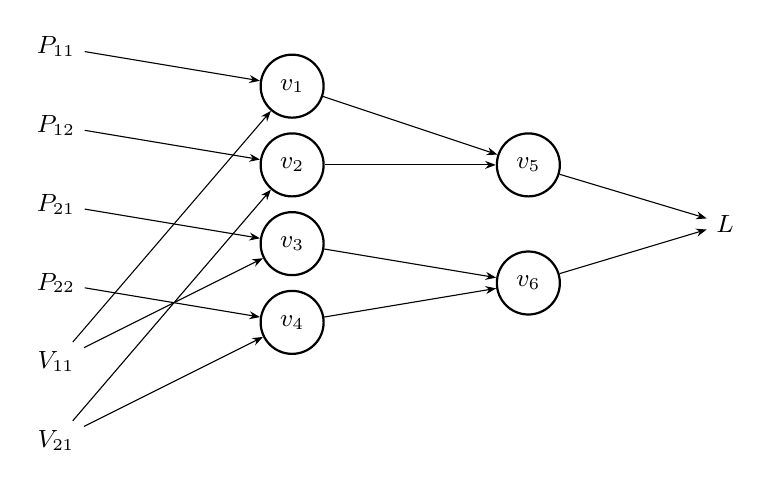
\begin{tikzpicture}[
  auto,
  intermediate/.style={draw,circle,minimum width=0.8cm,thick,font=\small},
  every label/.append style={font=\scriptsize}
]
  % Input labels (text only)
  \node[font=\small] (x1) at (0,3) {$P_{11}$};
  \node[font=\small] (x2) at (0,2) {$P_{12}$};
  \node[font=\small] (x3) at (0,1) {$P_{21}$};
  \node[font=\small] (x4) at (0,0) {$P_{22}$};
  \node[font=\small] (x5) at (0,-1) {$V_{11}$};
  \node[font=\small] (x6) at (0,-2) {$V_{21}$};

  % Intermediate nodes (v)
  \node[intermediate] (v1) at (3,2.5) {$v_1$};
  \node[intermediate] (v2) at (3,1.5) {$v_2$};
  \node[intermediate] (v3) at (3,0.5) {$v_3$};
  \node[intermediate] (v4) at (3,-0.5) {$v_4$};

  % Output nodes
  \node[intermediate] (v5) at (6,1.5) {$v_5$};
  \node[intermediate] (v6) at (6,0) {$v_6$};

  % Loss function
  \node[font=\small] (L) at (8.5,0.75) {$L$};

  % Forward edges
  \path[-{Stealth[scale=0.8]}]
    (x1) edge (v1)
    (x5) edge (v1)
    (x2) edge (v2)
    (x6) edge (v2)
    (x3) edge (v3)
    (x5) edge (v3)
    (x4) edge (v4)
    (x6) edge (v4)
    (v1) edge (v5)
    (v2) edge (v5)
    (v3) edge (v6)
    (v4) edge (v6)
    (v5) edge (L)
    (v6) edge (L);

\end{tikzpicture}
\end{center}
\end{frame}

\begin{frame}[allowframebreaks]
\frametitle{Computational Graph Node Values}
\begin{itemize}
\item Intermediate nodes represent element-wise products:
  \begin{align*}
    v_1 &= P_{11} \times V_{11} \\
    v_2 &= P_{12} \times V_{21} \\
    v_3 &= P_{21} \times V_{11} \\
    v_4 &= P_{22} \times V_{21} \\
    v_5 &= v_1 + v_2 = P_{11}V_{11} + P_{12}V_{21} = O_{11} \\
    v_6 &= v_3 + v_4 = P_{21}V_{11} + P_{22}V_{21} = O_{21}
  \end{align*}

\end{itemize}
\end{frame}

\begin{frame}[allowframebreaks]
\frametitle{Gradient w.r.t. V: Computational Graph ($\frac{\partial L}{\partial \mV}$)}
\begin{itemize}
\item $V_{11}$ affects $L$ through $v_1$ and $v_3$. Using chain rule:
\begin{align*}
\frac{\partial L}{\partial V_{11}} &= \frac{\partial L}{\partial v_5} \frac{\partial v_5}{\partial v_1} \frac{\partial v_1}{\partial V_{11}} + \frac{\partial L}{\partial v_6} \frac{\partial v_6}{\partial v_3} \frac{\partial v_3}{\partial V_{11}} \\[0.2cm]
&= \frac{\partial L}{\partial O_{11}} \cdot 1 \cdot P_{11} + \frac{\partial L}{\partial O_{21}} \cdot 1 \cdot P_{21} \\[0.2cm]
&= \sum_{i=1}^T P_{i1} \frac{\partial L}{\partial O_{i1}}
\end{align*}
\end{itemize}
\end{frame}

\begin{frame}[allowframebreaks]
\frametitle{Gradient w.r.t. V: Element-wise Operations ($\frac{\partial L}{\partial \mV}$)}

\vspace{1cm}
\begin{itemize}
\item Follow the same procedure for each element of $V$, we get:
  \begin{equation*}
    \frac{\partial L}{\partial V_{jk}} = \sum_{i=1}^T \frac{\partial L}{\partial O_{ik}} P_{ij}
  \end{equation*}

\item This is exactly the $(j,k)$-th element of matrix product
  \begin{equation*}
    \mP^\top \frac{\partial L}{\partial \mO}:
  \end{equation*}
  \begin{equation*}
    \left(\mP^\top \frac{\partial L}{\partial \mO}\right)_{jk} = \sum_{i=1}^T P_{ij} \frac{\partial L}{\partial O_{ik}}
  \end{equation*}

\item \textbf{Result}:
  \begin{equation*}
    \boxed{\frac{\partial L}{\partial \mV} = \mP^\top \frac{\partial L}{\partial \mO}}
  \end{equation*}
\end{itemize}
\end{frame}

\begin{frame}[allowframebreaks]
\frametitle{Gradient w.r.t. P ($\frac{\partial L}{\partial \mP}$)}
\begin{itemize}
\item From $O_{ik} = \sum_{j=1}^T P_{ij} V_{jk}$, we get:
  \begin{equation*}
    \frac{\partial L}{\partial P_{ij}} = \sum_{k=1}^d \frac{\partial L}{\partial O_{ik}} \frac{\partial O_{ik}}{\partial P_{ij}} = \sum_{k=1}^d \frac{\partial L}{\partial O_{ik}} V_{jk}
  \end{equation*}
\item In matrix form:
  \begin{equation*}
    \frac{\partial L}{\partial \mP} = \frac{\partial L}{\partial \mO} \mV^\top
  \end{equation*}
\end{itemize}
\end{frame}

\begin{frame}[allowframebreaks]
\frametitle{SoftMax Backward - The Two Paths}
\begin{itemize}
\item Now we need $\frac{\partial L}{\partial \mS}$ from $\frac{\partial L}{\partial \mP}$ through $\mP = \text{SoftMax}(\mS)$
\item Each $S_{ij}$ affects \textbf{ALL} probabilities in row $i$ due to normalization
\item For $P_{ij} = \frac{\exp(S_{ij})}{\sum_{k=1}^T \exp(S_{ik})}$, consider how $S_{ij}$ affects $P_{ik}$ for all $k$
\item \textbf{Two paths from $S_{ij}$ to loss $L$}:
  \begin{enumerate}
  \item \textbf{Direct path}: $S_{ij} \to P_{ij} \to L$
  \item \textbf{Normalization paths}: $S_{ij} \to P_{ik}$ (for $k \neq j$) $\to L$
  \end{enumerate}
\end{itemize}
\end{frame}

\begin{frame}[allowframebreaks]
\frametitle{SoftMax Gradient Calculation: Computational Graph}
\begin{itemize}
\item \textbf{Two computational paths for SoftMax gradients}:
\end{itemize}

\begin{center}
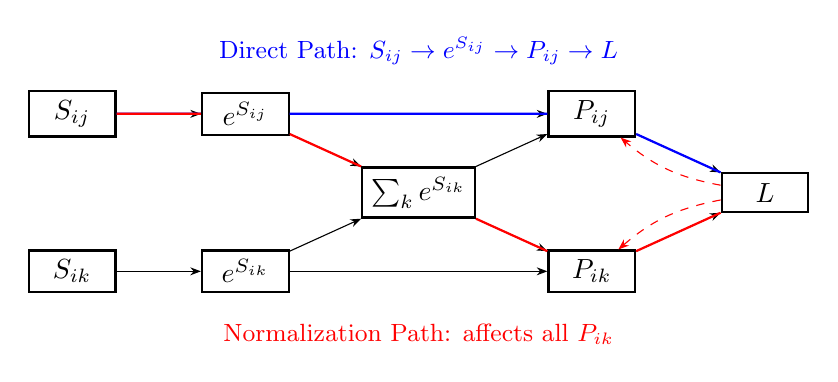
\begin{tikzpicture}[
  auto,
  vertex/.style={draw,rectangle,minimum width=1.1cm,minimum height=0.5cm,thick},
  every label/.append style={font=\small}
]
  % Input layer - attention scores (simplified)
  \node[vertex] (S) at (0,1) {$S_{ij}$};
  \node[vertex] (Sother) at (0,-1) {$S_{ik}$};

  % Exponential layer
  \node[vertex] (Exp) at (2.2,1) {$e^{S_{ij}}$};
  \node[vertex] (ExpOther) at (2.2,-1) {$e^{S_{ik}}$};

  % Normalization sum
  \node[vertex] (Sum) at (4.4,0) {$\sum_k e^{S_{ik}}$};

  % Probability layer
  \node[vertex] (P) at (6.6,1) {$P_{ij}$};
  \node[vertex] (POther) at (6.6,-1) {$P_{ik}$};

  % Loss
  \node[vertex] (L) at (8.8,0) {$L$};

  % Forward edges
  \path[-{Stealth[scale=0.8]}]
    (S) edge (Exp)
    (Sother) edge (ExpOther)
    (Exp) edge (Sum)
    (ExpOther) edge (Sum)
    (Exp) edge (P)
    (Sum) edge (P)
    (Sum) edge (POther)
    (ExpOther) edge (POther)
    (P) edge (L)
    (POther) edge (L);

  % Backward gradients (dashed)
  \path[-{Stealth[scale=0.8]},dashed,color=red]
    (L) edge[bend left=15] (P)
    (L) edge[bend right=15] (POther);

  % Path highlighting with simpler boxes
  \draw[color=blue, thick] (S) -- (Exp) -- (P) -- (L);
  \node[color=blue,font=\small] at (4.4,1.8) {Direct Path: $S_{ij} \to e^{S_{ij}} \to P_{ij} \to L$};

  \draw[color=red, thick] (S) -- (Exp) -- (Sum) -- (POther) -- (L);
  \node[color=red,font=\small] at (4.4,-1.8) {Normalization Path: affects all $P_{ik}$};
\end{tikzpicture}
\end{center}

\begin{itemize}
\item \textbf{Path 1 (Direct)}: $S_{ij} \to P_{ij} \to L$
  \begin{align}
    \frac{\partial P_{ij}}{\partial S_{ij}} &= P_{ij}(1 - P_{ij})
  \end{align}
\item \textbf{Path 2 (Normalization)}: $S_{ij} \to P_{ik} \to L$ for $k \neq j$
  \begin{align}
    \frac{\partial P_{ik}}{\partial S_{ij}} &= -P_{ij}P_{ik}
  \end{align}
\end{itemize}
\end{frame}

\begin{frame}[allowframebreaks]
\frametitle{SoftMax Gradient Calculation: Final Result}
\begin{itemize}
\item Combining both paths using chain rule:
  \begin{align}
    \frac{\partial L}{\partial S_{ij}} &= \frac{\partial L}{\partial P_{ij}} P_{ij}(1 - P_{ij}) + \sum_{k \neq j} \frac{\partial L}{\partial P_{ik}} (-P_{ij}P_{ik}) \\
    &= P_{ij} \left( \frac{\partial L}{\partial P_{ij}} - \sum_{k=1}^T \frac{\partial L}{\partial P_{ik}} P_{ik} \right)
  \end{align}
\end{itemize}
\end{frame}

\begin{frame}[allowframebreaks]
\frametitle{Gradient w.r.t. K}
\begin{itemize}
\item From $\mS = \mQ \mK^\top$, we have $S_{ij} = \sum_{\ell=1}^d Q_{i\ell} K_{j\ell}$
\item \textbf{Gradient w.r.t. K}:
  \begin{align}
    \frac{\partial L}{\partial K_{j\ell}} &= \sum_{i=1}^T \frac{\partial L}{\partial S_{ij}} \frac{\partial S_{ij}}{\partial K_{j\ell}} = \sum_{i=1}^T \frac{\partial L}{\partial S_{ij}} Q_{i\ell}
  \end{align}
\item In matrix form:
  \begin{equation*}
    \frac{\partial L}{\partial \mK} = \mQ^\top \frac{\partial L}{\partial \mS}
  \end{equation*}
\end{itemize}
\end{frame}

\begin{frame}[allowframebreaks]
\frametitle{Gradient w.r.t. Q}
\begin{itemize}
\item \textbf{Gradient w.r.t. Q}:
  \begin{align}
    \frac{\partial L}{\partial Q_{i\ell}} &= \sum_{j=1}^T \frac{\partial L}{\partial S_{ij}} \frac{\partial S_{ij}}{\partial Q_{i\ell}} = \sum_{j=1}^T \frac{\partial L}{\partial S_{ij}} K_{j\ell}
  \end{align}
\item In matrix form:
  \begin{equation*}
    \frac{\partial L}{\partial \mQ} = \frac{\partial L}{\partial \mS} \mK
  \end{equation*}
\end{itemize}
\end{frame}

\begin{frame}[allowframebreaks]
\frametitle{Assumptions for Backward Pass Algorithm}
\begin{itemize}
\item Intermediate matrices $\mP$, $\mS$ and $\frac{\partial L}{\partial \mO}$ are stored in HBM
\item The operations are done in blocks
\end{itemize}
\end{frame}

\begin{frame}[allowframebreaks]
\frametitle{Standard Attention Backward Algorithm}
\begin{itemize}
\item
  \begin{equation*}
    \frac{\partial L}{\partial \mV} = \mP^\top \frac{\partial L}{\partial \mO}
  \end{equation*}
\item
  \begin{equation*}
    \frac{\partial L}{\partial \mP} = \frac{\partial L}{\partial \mO} \mV^\top
  \end{equation*}
\item For $i = 1, \ldots, T$
  \begin{itemize}
  \item
    \begin{equation*}
      \text{sum} \leftarrow \left\langle \frac{\partial L}{\partial \mP_{i,:}}, P_{i,:} \right\rangle
    \end{equation*}
  \item For $j = 1, \ldots, T$
    \begin{itemize}
    \item
      \begin{equation*}
        \frac{\partial L}{\partial S_{ij}} \leftarrow P_{ij} \left( \frac{\partial L}{\partial P_{ij}} - \text{sum} \right)
      \end{equation*}
    \end{itemize}
  \end{itemize}
\item
  \begin{equation*}
    \frac{\partial L}{\partial \mK} = \mQ^\top \frac{\partial L}{\partial \mS}
  \end{equation*}
\item
  \begin{equation*}
    \frac{\partial L}{\partial \mQ} = \frac{\partial L}{\partial \mS} \mK
  \end{equation*}
\end{itemize}
\end{frame}

\begin{frame}[allowframebreaks]
\frametitle{Standard Attention Backward: Computational Complexity}
\begin{itemize}
\item \textbf{Step 1}:
  \begin{equation*}
    \frac{\partial L}{\partial \mV} = \mP^\top \frac{\partial L}{\partial \mO}
  \end{equation*}
  - $O(T^2 d)$ FLOPs
\item \textbf{Step 2}:
  \begin{equation*}
    \frac{\partial L}{\partial \mP} = \frac{\partial L}{\partial \mO} \mV^\top
  \end{equation*}
  - $O(T^2 d)$ FLOPs
\item \textbf{Step 3}: SoftMax backward computation - $O(T^2)$ FLOPs
\item \textbf{Step 4}:
  \begin{equation*}
    \frac{\partial L}{\partial \mK} = \mQ^\top \frac{\partial L}{\partial \mS} \quad \text{and} \quad \frac{\partial L}{\partial \mQ} = \frac{\partial L}{\partial \mS} \mK
  \end{equation*}
  - $O(T^2 d)$ FLOPs
\item \textbf{Overall complexity}: $O(T^2 d)$ operations
\end{itemize}
\end{frame}

\begin{frame}[allowframebreaks]
\frametitle{Standard Attention Backward: I/O Analysis}
\begin{itemize}
\item \textbf{Detailed I/O operations}:
  \begin{enumerate}
  \item \textbf{Load} $\mP \in \mathbb{R}^{T \times T}$ for computing
    \begin{equation*}
      \frac{\partial L}{\partial \mV}
    \end{equation*}
    $O(T^2)$ reads
  \item \textbf{Store}
    \begin{equation*}
      \frac{\partial L}{\partial \mP} \in \mathbb{R}^{T \times T}
    \end{equation*}
    $O(T^2)$ writes
  \item \textbf{Load} $\mP$ again for SoftMax backward computation: $O(T^2)$ reads
  \item \textbf{Load}
    \begin{equation*}
      \frac{\partial L}{\partial \mP}
    \end{equation*}
    for SoftMax backward: $O(T^2)$ reads
  \item \textbf{Store}
    \begin{equation*}
      \frac{\partial L}{\partial \mS} \in \mathbb{R}^{T \times T}
    \end{equation*}
    $O(T^2)$ writes
  \item \textbf{Load}
    \begin{equation*}
      \frac{\partial L}{\partial \mS}
    \end{equation*}
    for computing gradients w.r.t. $\mK$ and $\mQ$: $O(T^2)$ reads
  \end{enumerate}
\item \textbf{Total I/O cost}: $6 \times O(T^2) = O(T^2)$ memory accesses
\item \textbf{Performance bottleneck}:
  \begin{itemize}
  \item Computation: $O(T^2 d)$ FLOPs
  \item Memory access: $O(T^2)$ elements
  \item \textbf{When $d$ is small}: memory access dominates!
  \end{itemize}
\item The $T \times T$ attention matrix is the bottleneck for both forward and backward passes
\end{itemize}
\end{frame}


\begin{frame}[allowframebreaks]
	\frametitle{References}
	\begin{scriptsize}
		\def\newblock{}
		\bibliographystyle{abbrvnat}
		\bibliography{references}
	\end{scriptsize}
\end{frame}

\end{document}


%%% Local Variables:
%%% mode: latex
%%% TeX-master: t
%%% End:
